%!TEX root = ../notes.tex
\section{February 3, 2025}
\label{20250203}

\subsection{Message Integrity}

Last lecture, we touched upon methods of authenticating a message. The symmetric-key version is called a MAC (message authentication code), the public-key version is called a digital signature. Let's review what we covered last time.

\subsubsection{Message Authentication Code}
To authenticate a message, Alice will use the private key $k$ to tag a message $m$ with a tag $t$. Bob will verify that $(m, t)$ is valid with key $k$.

\Graphic{images/2023-02-07/mac.png}{0.7}

\subsubsection{Digital Signature}
\label{sec:feb7-ds}
Similarly we have the public-key version. Alice has a secret key $sk$ to sign message $m$ with signature $\sigma$. Bob (or anyone) can verify with the public key $pk$ that $(m, \sigma)$ is a valid signature.

\Graphic{images/2023-02-07/ds.png}{0.7}

\subsubsection{Syntax}
Recall the syntax of MAC and digital signatures (see \cref{sec:message-integrity:syntax}).

A message authentication code (MAC) scheme consists of $\Pi = (\Gen, \mathsf{Mac}, \mathsf{Verify})$.
\begin{description}
    \item[Generation.] $k\leftarrow \Gen(1^\lambda)$.
    \item[Authentication.] $t \leftarrow \mathsf{Mac}_k(m)$.
    \item[Verification] $0/1 := \mathsf{Verify}_k(m, t)$.
\end{description}

A digital signature scheme consists of $\Pi = (\Gen, \mathsf{Sign}, \mathsf{Verify})$.
\begin{description}
    \item[Generation.] $(sk, vk)\leftarrow \Gen(1^\lambda)$.
    \item[Authentication.] $\sigma \leftarrow \mathsf{Sign}_{sk}(m)$.
    \item[Verification] $0/1 := \mathsf{Verify}_{vk}(m, \sigma)$.
\end{description}

\subsubsection{Chosen-Message Attack}
Similar to chosen-plaintext attack from encryption, we have chosen-message attack security. An adversary chooses a number of messages to generate signatures or tags for. After that, the adversary will try to generate another valid pair of message and tag. We want to make sure that generating a new pair of message and tag is extremely hard (negligible probability of success).

\begin{center}
    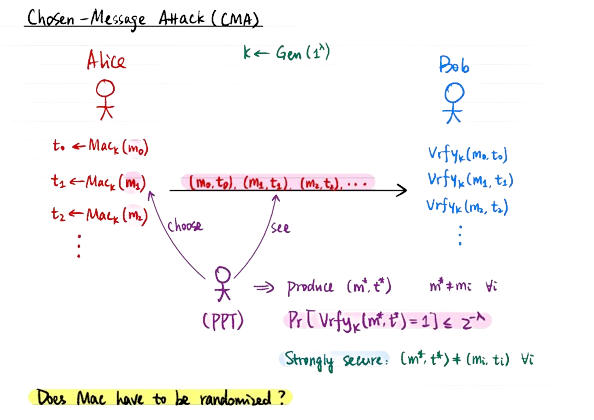
\includegraphics[width=0.8\textwidth]{images/2023-02-02/cma.png}
\end{center}

\begin{center}
    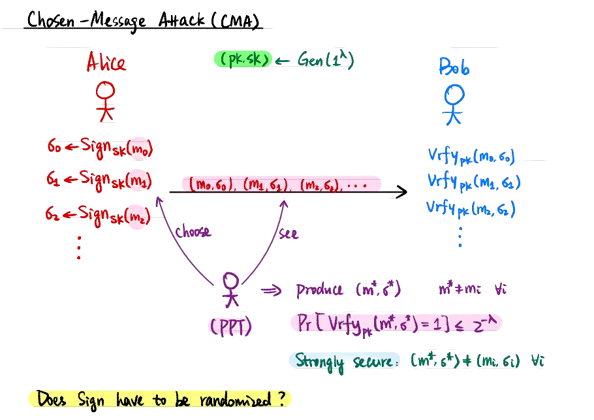
\includegraphics[width=0.8\textwidth]{images/2023-02-02/cma2.png}
\end{center}

\begin{ques*}
    Do the MAC and signature algorithms need to be randomized to be CMA secure?
\end{ques*}
No! Unlike CPA security, we don't need these algorithms to be randomized to be CMA secure. It is ok for these algorithms to be deterministic, since it is still difficult for an adversary to produce a \emph{new} message-signature pair.

% \subsubsection{Constructions}
% We can construct MAC pratically using
% \begin{itemize}
%     \item Block Cipher: CBC-MAC
%     \item Hash Functions: HMAC
% \end{itemize}

% We can construct digital signatures using
% \begin{itemize}
%     \item RSA signature: RSA Assumption.
%     \item DSA signature: Discrete Log Assumption
%     \item Lattice-Based Encryption Schemes (post-quantum secure).
% \end{itemize}

\subsection{RSA Signatures}
Our RSA signatures algorithm works very similarly to RSA encryption.

We generate two $n$-bit primes $p, q$. Compute $N:=p\cdot q$ and $\phi(N) = (p-1)(q-1)$. Again choose $e$ with $\gcd(e, \phi(N)) = 1$ and invert $d = e^{-1}\mod\phi(N)$. Given $N$ and a random $y\sampledfrom\ZZ_N^\times$, it's computationally hard to find $x$ such that $x^e\equiv y\mod N$.

Similarly, $sk := d$ and $vk := (N, e)$. To sign, we compute
\[\Sign_{sk}(m) := m^d\mod{N}.\]
To verify, we compute
\[\Verify_{vk}(m, \sigma):= \sigma^e\overset{?}{\equiv}m\mod N.\]

\begin{ques*}
    Are there any security issues with RSA as we have constructed it so far?
\end{ques*}

Yes, there are several attacks that can be leveraged. A simple on is to sample some $\sigma^* \in \ZZ_N^*$, and then compute $m^* := (\sigma^*)^e$.

Attacks can be more targeted. If Eve knows many messages and signatures, she can compute another pair of valid message and keys. If we have messages
\begin{align*}
    m_0, \sigma_0 & = m_0^d\mod N \\
    m_1, \sigma_1 & = m_0^d\mod N
\end{align*}
We can compute $m^* := m_0\cdot m_1$ and $\sigma^* := \sigma_0 \cdot \sigma_1 = (m_0\cdot m_1)^d\mod N$.

We can do linear combinations of messages, as well as raising messages to arbitrary exponents, and we can get other messages with valid signatures.

There is an easy solution, however. We can hash our message $m$ before we sign, like so
\begin{align*}
    \Sign_{sk}(m)           & := {\color{red}H(}m{\color{red})}^d\mod{N}                         \\
    \Verify_{vk}(m, \sigma) & := \sigma^e\overset{?}{\equiv}{\color{red}H(}m{\color{red})}\mod N
\end{align*}
where $H$ is a hash function\footnote{A hash function is, briefly, a function that produces some random output that is hard to compute the inverse of.}. This is a commonly known technique called `hash-and-sign'.

\subsubsection{Other Signature Schemes}

There are also other signature schemes that rely on other hardness assumptions.

\begin{itemize}
    \item RSA signatures rely on the RSA assumption.
    \item Schnorr/DSA signatures rely on the discrete log assumption.
    \item Lattice-based encryption schemes are post-quantum secure and rely on the hardness of certain lattice problems.
\end{itemize}

\subsection{A Summary So Far}
\label{sec:feb7-summary-so-far}
To summarize, here's all we've covered so far:
\begin{center}
    \begin{tabular}{@{}lll@{}}
        \toprule
                                      & \textbf{Symmetric-Key}                                                                & \textbf{Public-Key}                                                                   \\ \midrule
        \textbf{Message Secrecy}      & \begin{tabular}[c]{@{}l@{}}Primitive: SKE\\ Construction: Block Cipher\end{tabular}    & \begin{tabular}[c]{@{}l@{}}Primitive: PKE\\ Constructions: RSA/ElGamal\end{tabular}   \\ \midrule
        \textbf{Message Integrity}    & \begin{tabular}[c]{@{}l@{}}Primitive: MAC\\ Constructions: CBC-MAC/HMAC\end{tabular}   & \begin{tabular}[c]{@{}l@{}}Primitive: Signature\\ Constructions: RSA/DSA\end{tabular} \\ \midrule
        \textbf{Secrecy \& Integrity} & \begin{tabular}[c]{@{}l@{}}Primitive: AE\\ Construction: Encrypt-then-MAC\end{tabular} &                                                                                       \\ \midrule
        \textbf{Key Exchange}         &                                                                                        & Construction: Diffie-Hellman                                                          \\ \midrule
        \textbf{Important Tool}                & \begin{tabular}[c]{@{}l@{}}Primitive: Hash function\\ Construction: SHA\end{tabular}   &                                                                                       \\ \bottomrule
    \end{tabular}
\end{center}

\subsection{Authenticated Encryption}
\label{sec:feb7-authenticated-encryption}
Generally, Alice and Bob will first perform a Diffie-Hellman key exchange, then use that shared key to conduct Symmetric-Key Encryption.

\Graphic{images/2023-02-07/practice.png}{0.6}

In reality, we want to achieve both message secrecy and integrity \emph{at the same time}. For this, we can introduce Authenticated Encryption.

Our security definition is that our adversary can see the encryptions of many messages $m_0, m_1, m_2$. We want \textbf{CCA security}: that an adversary given previous ciphertexts and their decryptions cannot distinguish between the encryptions of a fresh pair of messages $m_0$ and $m_1$. \emph{Additionally}, we want the property of \textbf{unforgeability}, that our adversary cannot generate a $c^*$ that is a valid encryption, such that $\Dec_{k}(c^*)\neq m_i$ for any $i$.

\begin{definition}[Chosen Ciphertext Attack]
    An adversary is allowed to query any number of messages, and receives their corresponding ciphertexts. The adversary can also request decryptions from a decryption oracle for any ciphertext, and will see the resulting decryption.
\end{definition}

\begin{definition}[Unforgeability]
    An adversary can query any message. They are unable to create a new message that has not been queried before, and which can be authenticated. 
\end{definition}

\Graphic{images/2023-02-07/ae.png}{0.8}

Now that we have two new primitives, we can construct Authenticated Encryption schemes.

\begin{remark}
    This section describes three different approaches to AE: Encrypt-and-MAC, Encrypt-then-MAC, and MAC-then-Encrypt. In practice, only Encrypt-then-MAC satisfies CCA security and unforgeability. The other approaches are provided as counterexamples.
\end{remark}

\subsubsection{Encrypt-and-MAC?}
Given a CPA-secure SKE scheme $\Pi_1(\Gen_1, \Enc_1, \Dec_1)$ and a CMA-secure MAC scheme $\Pi_2 = (\Gen_2, \Mac_2, \Verify_2)$.

We construct an AE scheme $\Pi = (\Gen, \Enc, \Dec)$ by composing encryption and MAC. We encrypt the plaintext and also compute the MAC the \emph{plaintext}.

\Graphic{images/2023-02-07/encrypt-and-mac.png}{0.3}

\begin{description}
    \item[$\Gen(1^\lambda)$:] $k_1:=\Gen_1(1^\lambda)$, $k_2:=\Gen_2(1^\lambda)$, output $(k_1, k_2)$.

    \item[$\Enc(m)$:] To encrypt, we first encrypt ciphertext $c_1 := \Enc_1(k_1, m)$ and sign message (in plaintext) $t_2 := \Mac_2(k_2, m)$ and output $(c_1, t_2)$.

    \item[$\Dec(m)$:] We have ciphertext $c = (c_1, t_2)$. Our message is $m:=\Dec_1(k_1, c_1)$, and our verification bit $b := \Verify_1(k_2, (m, t_2))$. If $b = 1$, output $m$, otherwise we output $\bot$.
\end{description}

\begin{ques*}
    Is this scheme secure? Assuming the CPA-secure SKE scheme and CMA-secure MAC scheme, does this give us both CPA-security and unforgeability?
\end{ques*}

MAC gives you \emph{unforgeability}---but it doesn't even try to hide the message at all. It's possible that the MAC scheme reveals the message in the clear. For example, we might have a MAC scheme that includes the message in the signature \emph{in the clear} (which is still secure)!

Since MAC doesn't try to hide the message. If our MAC reveals something about our message, our composed scheme $\Pi$ doesn't give us CPA-security. You might still be able to infer something about the message.

We try something else\dots

\subsubsection{MAC-then-Encrypt?}
Similarly, we can also MAC first, encrypt the entire ciphertext and tag concatenated.

\Graphic{images/2023-02-07/mac-then-encrypt.png}{0.3}

\begin{description}
    \item[$\Gen(1^\lambda)$:] $k_1:=\Gen_1(1^\lambda)$, $k_2:=\Gen_2(1^\lambda)$, output $(k_1, k_2)$.

    \item[$\Enc(m)$:] To encrypt, we first encrypt ciphertext $c_1 := \Enc_1(k_1, m)$ and sign message (in plaintext) $t_2 := \Mac_2(k_2, {\color{red} m||t_2})$ and output $(c_1, t_2)$.

    \item[$\Dec(m)$:] We have ciphertext $c = (c_1, t_2)$. Our message is ${\color{red} m||t_2}:=\Dec_1(k_1, c_1)$, and our verification bit $b := \Verify_1(k_2, (m, t_2))$. If $b = 1$, output $m$, otherwise we output $\bot$.
\end{description}

\begin{ques*}
    Is this secure?
\end{ques*}

This doesn't satisfy a stronger security definition called Chosen Ciphertext Attack (CCA) security. We might be able to forge ciphertexts that decrypt to valid message and tags.

\subsubsection{Chosen Ciphertext Attack Security}
On top of CMA security, the adversary can now request Alice to decrypt ciphertexts $c_0, c_1, \dots$. 

\Graphic{images/2023-02-07/cca.png}{0.7}

We can prove that MAC-then-Encrypt is not CCA secure.

\subsubsection{Encrypt-then-MAC}
We encrypt first, then we MAC on the \emph{ciphertext}.

\Graphic{images/2023-02-07/encrypt-then-mac.png}{0.3}

\begin{description}
    \item[$\Gen(1^\lambda)$:] $k_1:=\Gen_1(1^\lambda)$, $k_2:=\Gen_2(1^\lambda)$, output $(k_1, k_2)$.

    \item[$\Enc(m)$:] To encrypt, we first encrypt ciphertext $c_1 := \Enc_1(k_1, m)$ and sign message (in ciphertext) $t_2 := \Mac_2(k_2, {\color{red} c_1})$ and output $(c_1, t_2)$.

    \item[$\Dec(m)$:] We have ciphertext $c = (c_1, t_2)$. Our message is $m:=\Dec_1(k_1, c_1)$, and our verification bit $b := \Verify_1(k_2, ({\color{red} c_1}, t_2))$. If $b = 1$, output $m$, otherwise we output $\bot$.
\end{description}

You can prove that Encrypt-then-MAC schemes are CPA-secure and unforgeable. In addition, Encrypt-then-MAC is CCA secure, since our decryption oracle will not decrypt if the ciphertext cannot be verified, meaning only valid ciphertext-tag pairs can be passed.

The moral of this is that \textbf{you should always use Encrypt-then-MAC.}

\subsection{Hash Function}
A hash function is a public function
\[H: {0, 1}^*\to {0, 1}^n\]
where $n$ is order $\Theta(\lambda)$.

\Graphic{images/2023-02-07/hash.png}{0.5}

We want our hash function to be collision-resistant. That is, it's computationally hard to find $x, y\in\left\{ 0, 1 \right\}^*$ such that $x\neq y$ yet $H(x) = H(y)$ (which is called a collision).

More to come next class!